\documentclass[a4paper,10pt,oneside]{book}

% packages 
\usepackage{arsclassica}    % fancy layout
\usepackage[english]{babel}\addto{\captionsenglish}{\renewcommand{\bibname}{References}}
\usepackage{caption}         % figure captions
\usepackage[square,numbers,super,sort&compress]{natbib}  % bibliography style
\usepackage[cc]{titlepic}    % enable logo on title page
\usepackage{graphicx}       % logo related
\usepackage{float} 

\usepackage{standalone}

% bibliography
\bibliographystyle{../thesis}

% title setup
\title{ \vspace{3in} Unravelling higher order genome organisation {\small [working
    title]} \\ \vspace{2em} {\large {\bf Introduction}} }
\author{Benjamin L. Moore}
\titlepic{\vspace{2.2in} 
\includegraphics[width=\textwidth]{/Users/benmoore/hvl/1yrReport/figs/igmm.png}}

\begin{document}

\maketitle

\chapter{Reanalysis of Hi-C datasets}

\section{Introduction}

Since the initial publication of the Hi-C technique in 2009,\cite{Lieberman2009} there has been rapid advancement of both the technique itself and the resolution at which interaction frequencies have been analysed. From the proof-of-concept analysis at 1 megabase (Mb) and 100 killable (kb) resolution,\cite{Lieberman2009} subsequent experiments achieved first 40 kb\cite{Dixon2012}, then 10 kb\cite{Jin2013} and most recently 1 kb\cite{Rao2014}, enabling bona fide fragment-level analysis for the first time.

% timeline: 
% Lieberman Aiden 2009       1 Mb (30 M reads)
% Dixon 2012                       40 kb (300 M reads)
% Jin 2013                        5-10 kb ()
% Rao 2014                           1 kb

Such rapid progression in the field has resulted in a wide variety of public Hi-C datasets being available, albeit with differing qualities. With proper correction and at a suitable resolution, these interaction frequencies can be compared and contrasted within and between species.

In this work I uniformly reprocessed publicly-available human Hi-C datasets, in order to address fundamental questions about the stability of higher order genome organisation within cell populations from the same species. Previously Hi-C studies have compared two samples per species, such as K562 against GM06990\cite{Lieberman2009} or IMR90 against GM12878.\cite{Dixon2012} Here I make use of three Hi-C datasets corresponding to extensively-studied human cell lines: K562, GM12878 and H1 hESC. Together these make up the "Tier 1" cell lines studied by the ENCODE consortium,\cite{Dunham2012} hence have huge amounts of matched ChIP-seq and histone modification data available. 

By combinatorial reanalysis of these cell-matched datasets, I can investigate t

% Table: description of cell lines

\section{Hi-C reprocessing}

Each Hi-C dataset used in this work was reprocessed using the same pipeline from raw sequencing reads. In each case, experiments used the same HindIII restriction enzyme.

% Pipeline:
% 1. iterative mapping
% 2. 

% figure showing contact maps, before and after (split cell type?)

\section{Compartment profiles}
% how well do compartments correlate

After uniformly reprocessing each Hi-C dataset and calling compartment eigenvector profiles (see \emph{Methods}), we can compare these between three human cell lines. Compartment profiles have a visibly high-correspondence (Fig. \ref{fig:wiggles}), despite the variable sources of both sample material and experimental data.

\begin{figure}
\begin{center}
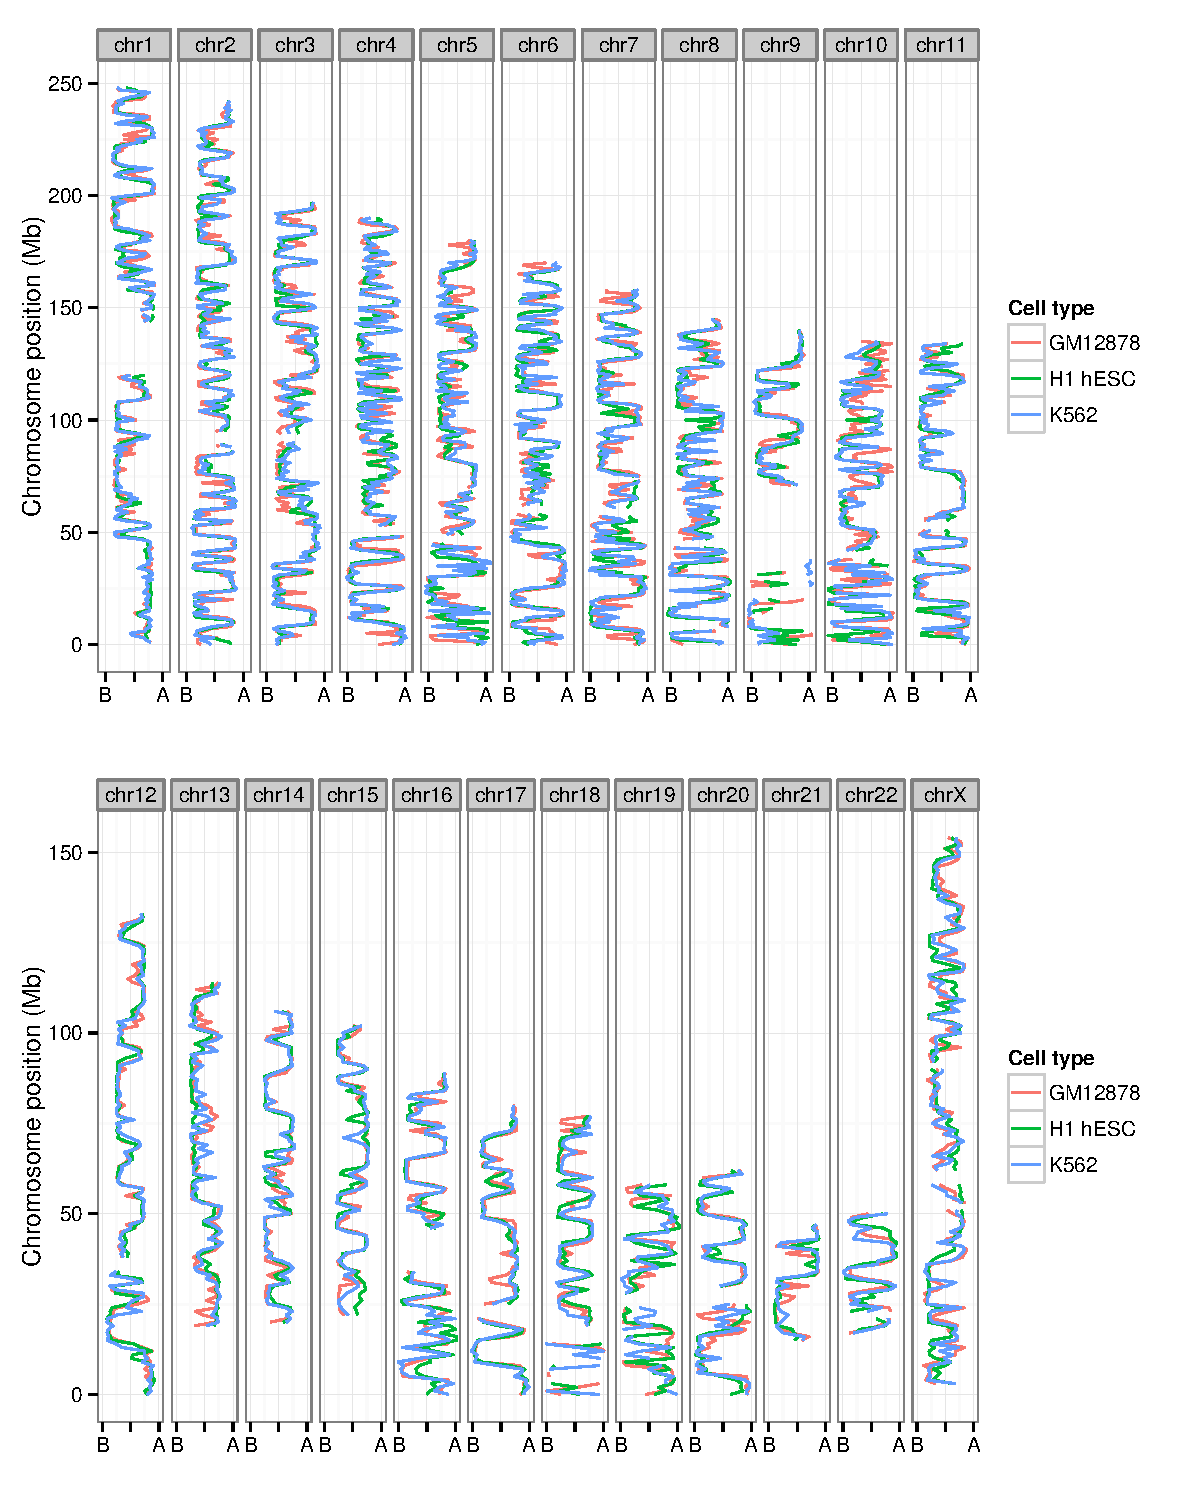
\includegraphics[width=1.2\textwidth]{figs/wiggles.pdf}
\captionsetup{width=\textwidth}
\caption{
{\bf Compartment profiles are observably well-correlated between human cell types and across all chromosomes.}
Caption
}\label{fig:wiggles}
\end{center}
\end{figure} 

This close correspondence also validates our approach of combining these different datasets, and suggests our uniform pipeline is successfully accounting for differences in sequencing depth and other batch effects. The precise correlations of these independent measures are in the interval $R = [.75, .8]$ (Fig. \ref{fig:compactor}; Pearson correlation coefficients, PCC).

\begin{figure}
\begin{center}
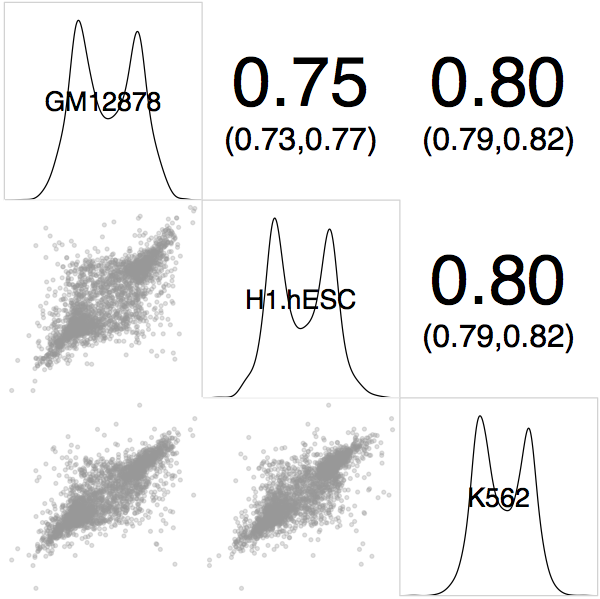
\includegraphics[width=.5\textwidth]{figs/compartment_corr.png}
\captionsetup{width=\textwidth}
\caption{
{\bf Compartment eigenvectors are well-correlated between human cell types}
Megabase resolution compartment eigenvector values are shown in a plot matrix. \emph{Upper triangle}: Pearson correlation coefficients between pairs, with $95\%$ confidence intervals (??); \emph{diagonal} Kernel density estimates of eigenvector values per cell type; \emph{lower triangle}: $x$-$y$ scatterplot of values.
}\label{fig:compcor}
\end{center}
\end{figure} 

\section{Domain calls}

The continuous compartment eigenvector can be used as-is to classify A/B compartments, using positive and negative eigenvector values after first orientating the vector with respect to, for example, PolII Chip-seq data.\cite{Kalhor2012} However, given the definition of compartments as generally broad and alternating domains along a chromosome, often matching other large domains of Lamin association, an improved classification method might penalise the calls of short compartment calls, which may be the result of noise.

For this reason, instead of using raw eigenvector values we consider observed values as emissions from unobserved underlying states. This can be modelled through a Hidden Markov Model (HMM), whereby we first parameterise models of state and their transitions, then infer the most likely state sequence to have emitted our observed data. This unobserved two-state sequence is then used for compartment calls. 

In practice, this acts to de-noise our compartment calls. Where single sign-changes along the series would have resulted in a single-block compartment, these may now be modelled as noisy emissions from a single unobserved state. An examplar region is showing in Fig. \ref{fig:denoise}.

% figure showing raw eigs with hmm calls
\begin{figure}
\begin{center}
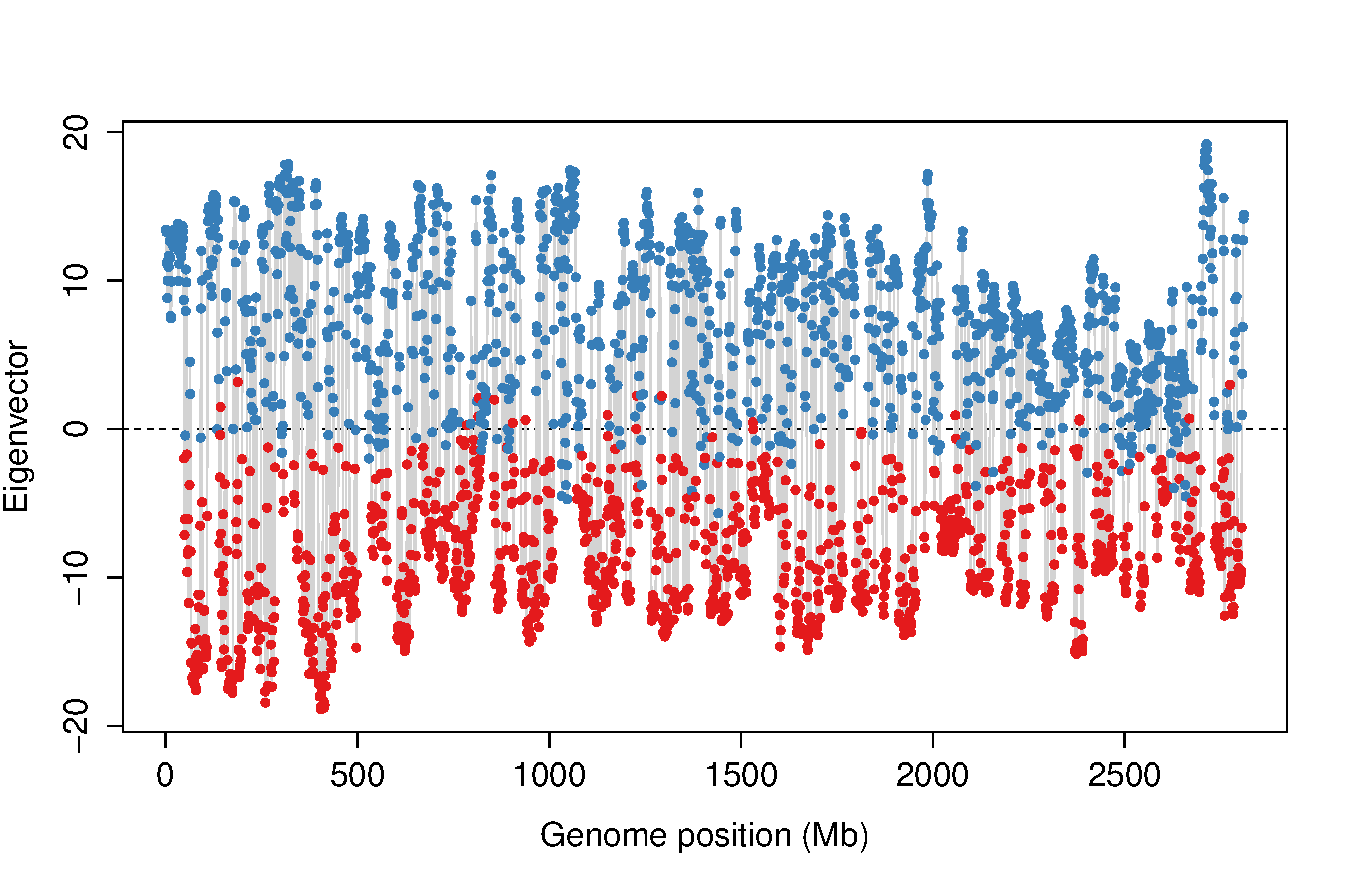
\includegraphics[width=.9\textwidth]{figs/hmm_denoise.pdf}
\captionsetup{width=\textwidth}
\caption{
{\bf ??}
placeholder 
}\label{fig:denoise}
\end{center}
\end{figure} 

% figure showing size distributions of Hi-C domains

\section{Variable regions}
% investigate those regions which are "flipped"

Despite the vast majority of the genome being in matched chromatin compartments, there are also regions of disagreement. Reasons for observable differences include technical errors and bias, but also more interesting functional explanations, where cell-type specific activation or repression is reflected in changes in higher order structure.








% fig 1.

\section{Nuclear positioning}



\ifstandalone
\begin{small}
\bibliography{/Users/benmoore/Documents/library,/Users/benmoore/Documents/customrefs}
\end{small}
\fi

\end{document}
